
\begin{frame}{Componente SeekBar en Android}
\textbf{¿Qué es un SeekBar?}

\begin{itemize}
    \item Es un componente de interfaz gráfica que permite al usuario seleccionar un valor dentro de un rango deslizando un control horizontal.
    \item Es una extensión de la clase ProgressBar con interacción del usuario.
\end{itemize}

\vspace{0.5cm}

\textbf{¿Para qué sirve?}
\begin{itemize}
    \item Ajustar valores continuos o discretos (ej. volumen, brillo, progreso).
    \item Permitir entrada intuitiva mediante deslizamiento.
    \item Controlar parámetros en tiempo real.
\end{itemize}

\vspace{0.5cm}

\textbf{Características principales:}
\begin{itemize}
    \item Permite definir valores mínimo, máximo y progreso actual.
    \item Puede escuchar cambios mediante un listener (OnSeekBarChangeListener).
    \item Es altamente personalizable (colores, tamaño, estilo).
\end{itemize}


\end{frame}


\begin{frame}[fragile]
\frametitle{Demo 08: Agregar SeekBars}
\begin{columns}
\column{0.80\linewidth}
Del Repositorio Github:
\begin{itemize}
\item Copiar el archivo MainActivity\_Demo08.java (dentro del Folder códigosJAVA) al mismo directorio donde esta el MainActivity.java
\item Copiar el archivo activity\_main\_demo08.xml (dentro del Folder Carpeta\_layout) al mismo directorio donde esta el activity\_main.xml
%\item Copiar los archivos \textit{cgup.jpg} y \textit{logo\_upv\_2019.png} localizados dentro de la folder \textit{Carpeta\_drawable} en el directorio \textit{res/drawable} del proyecto de AS.
\item Modificar en el archivo AndroidManifest.xml la cadena \textit{.MainActivity\_Demo07} por \textit{.MainActivity\_Demo08}
\end{itemize}

\begin{block}{Demo \#08}
Muestra una App dos SeekBars (la segunda utiliza separadores finitos). La primera SeekBar actualiza el contenido de TextView conforme la seleccion del usuario. 
\end{block}


\column{0.20\linewidth}

\begin{center}
 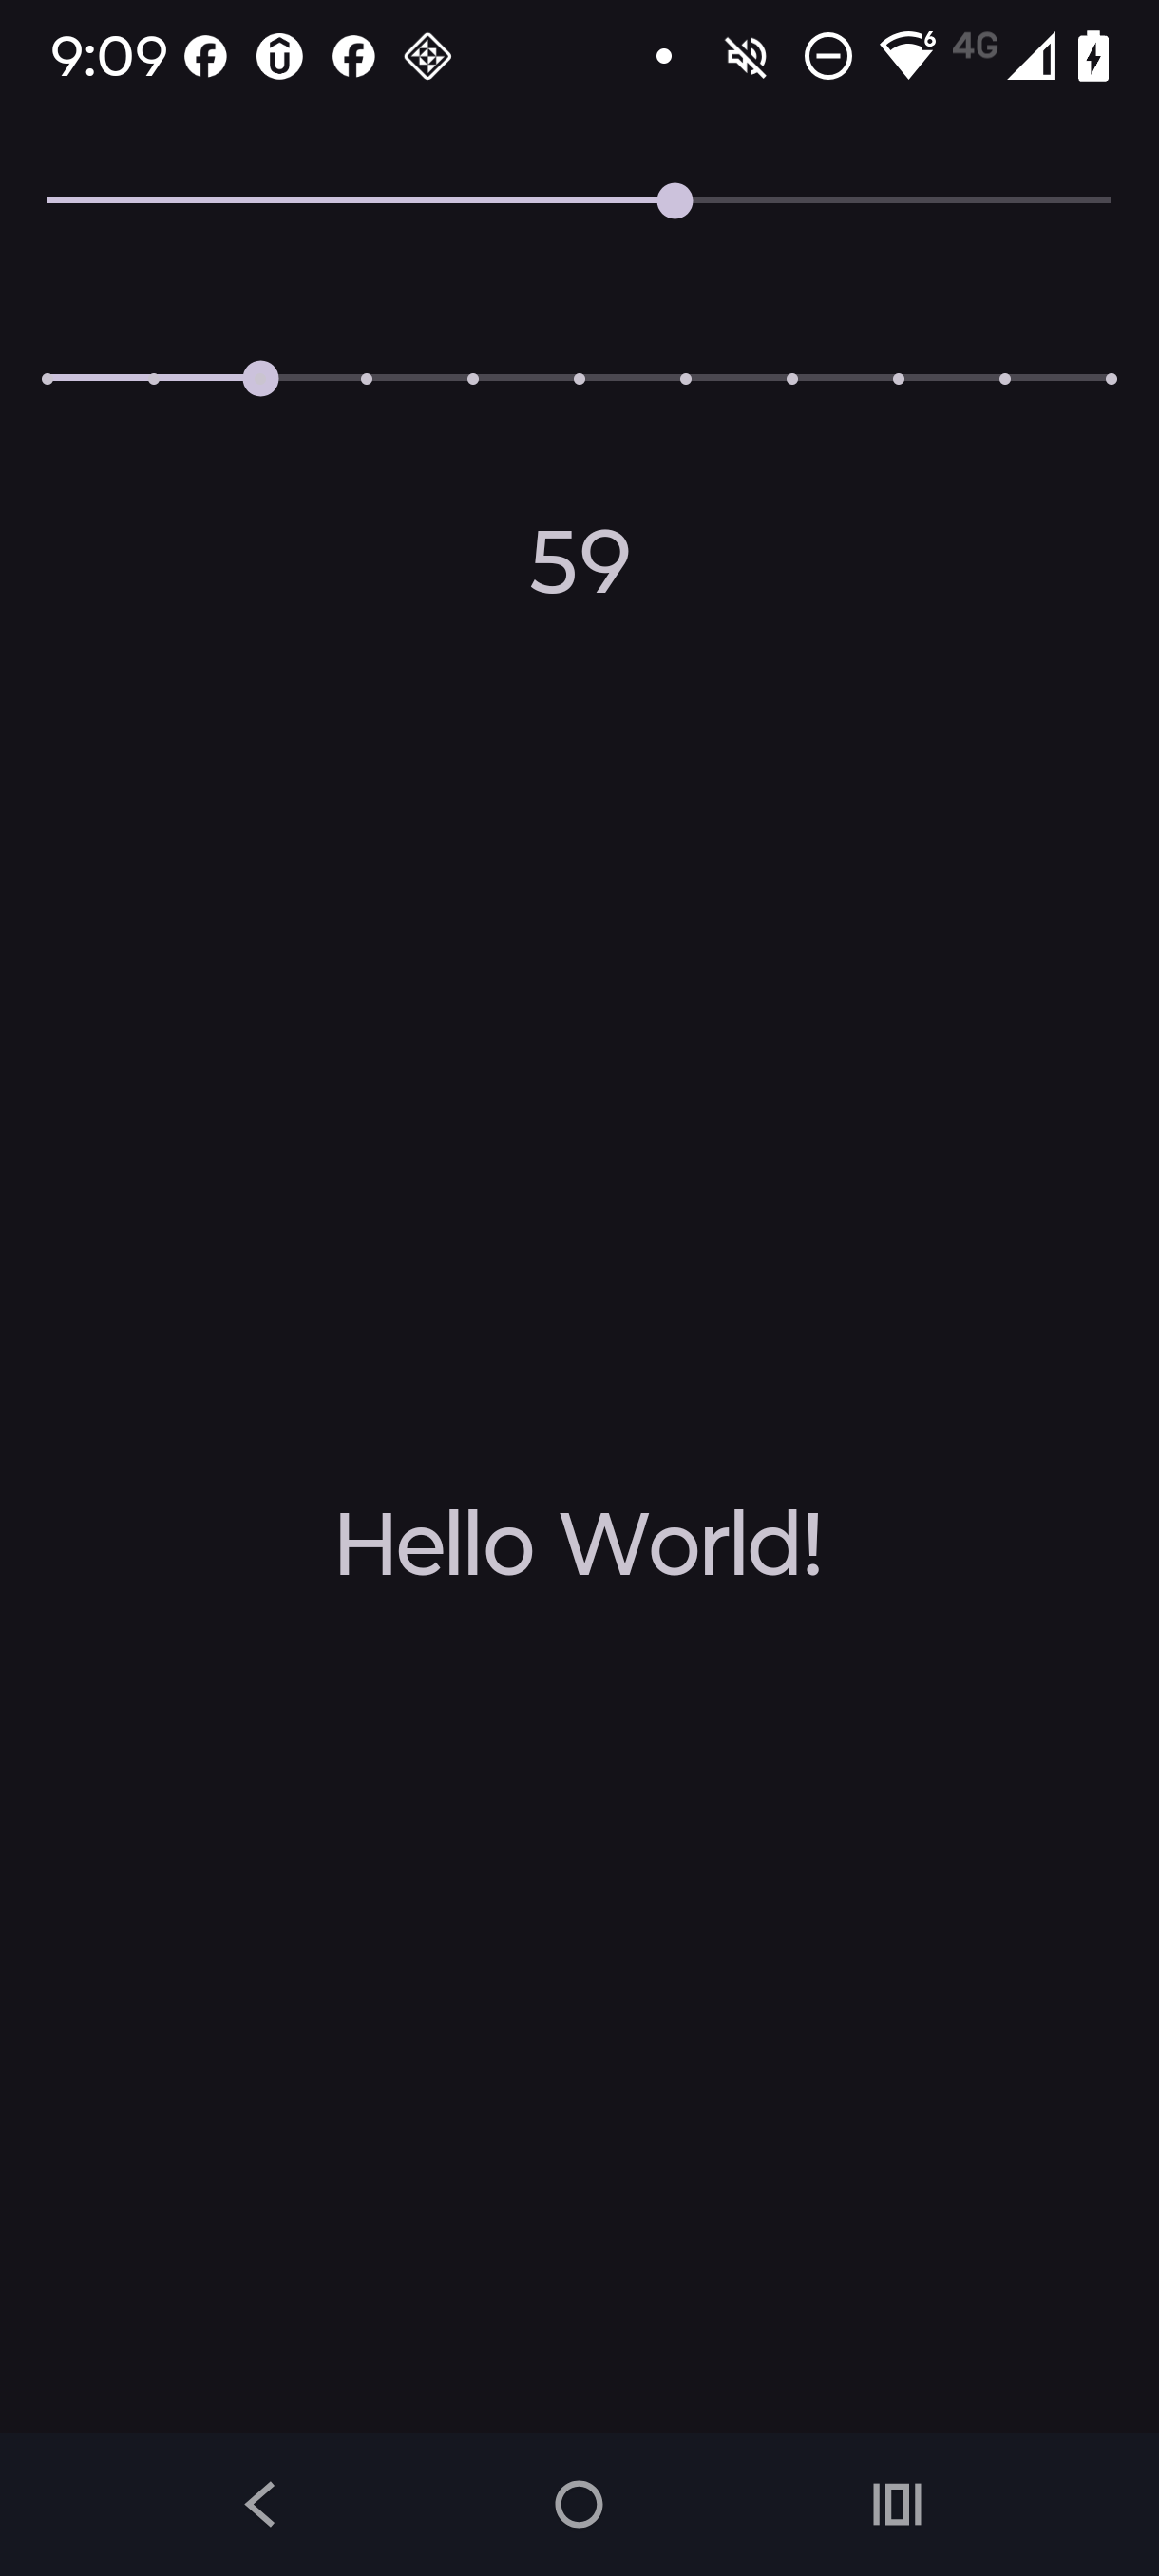
\includegraphics[width=0.98\textwidth]{02_TallerCBTis/figs/Demo08}
\end{center}

\end{columns}

\end{frame}


